\documentclass{beamer}

\mode<presentation> {
}

\title[]{Bayesian Clinical Trials} 
\subtitle{Informative vs. non-informative beta priors} 
\date{} 

\usepackage{graphicx} 
\usepackage{booktabs} 
\usepackage{longtable} 
 \usepackage{hyperref}


\usepackage{color}
\usepackage{fancyvrb}

\definecolor{shadecolor}{gray}{1.00}

\DefineShortVerb[commandchars=\\\{\}]{\|}
\DefineVerbatimEnvironment{Highlighting}{Verbatim}{commandchars=\\\{\}}
\newenvironment{Shaded}{}{}
\newcommand{\KeywordTok}[1]{\textcolor[rgb]{0.00,0.44,0.13}{\textbf{{#1}}}}
\newcommand{\DataTypeTok}[1]{\textcolor[rgb]{0.56,0.13,0.00}{{#1}}}
\newcommand{\DecValTok}[1]{\textcolor[rgb]{0.25,0.63,0.44}{{#1}}}
\newcommand{\BaseNTok}[1]{\textcolor[rgb]{0.25,0.63,0.44}{{#1}}}
\newcommand{\FloatTok}[1]{\textcolor[rgb]{0.25,0.63,0.44}{{#1}}}
\newcommand{\CharTok}[1]{\textcolor[rgb]{0.25,0.44,0.63}{{#1}}}
\newcommand{\StringTok}[1]{\textcolor[rgb]{0.25,0.44,0.63}{{#1}}}
\newcommand{\CommentTok}[1]{\textcolor[rgb]{0.38,0.63,0.69}{\textit{{#1}}}}
\newcommand{\OtherTok}[1]{\textcolor[rgb]{0.00,0.44,0.13}{{#1}}}
\newcommand{\AlertTok}[1]{\textcolor[rgb]{1.00,0.00,0.00}{\textbf{{#1}}}}
\newcommand{\FunctionTok}[1]{\textcolor[rgb]{0.02,0.16,0.49}{{#1}}}
\newcommand{\RegionMarkerTok}[1]{{#1}}
\newcommand{\ErrorTok}[1]{\textcolor[rgb]{1.00,0.00,0.00}{\textbf{{#1}}}}
\newcommand{\NormalTok}[1]{{#1}}

\hypersetup{breaklinks=true, pdfborder={0 0 0}}
\setlength{\parindent}{0pt}
\setlength{\parskip}{6pt plus 2pt minus 1pt}
\setlength{\emergencystretch}{3em}  
\setcounter{secnumdepth}{0}
%\EndDefineVerbatimEnvironment{Highlighting}








\begin{document}



\begin{frame}
\titlepage % Print the title page as the first slide
\end{frame}


\begin{frame}[fragile]{Updatindg with Data}

\begin{Shaded}
\begin{Highlighting}[]
\KeywordTok{library}\NormalTok{(LearnBayes)}
\end{Highlighting}
\end{Shaded}

Suppose we are interested in the response \(p\) of a drug.

\begin{itemize}
\item
  The function \textbf{bayes.select} allow for specifying a beta prior
  based on knowledge of two prior quantiles.
\item
  Suppose the prior median for the response rate is 0.2 and the 75th
  percentile is 0.3.
\end{itemize}

\begin{Shaded}
\begin{Highlighting}[]
\NormalTok{beta.prior =}\StringTok{ }\KeywordTok{beta.select}\NormalTok{(}\KeywordTok{list}\NormalTok{(}\DataTypeTok{p=}\FloatTok{0.5}\NormalTok{, }\DataTypeTok{x=}\FloatTok{0.2}\NormalTok{), }\newline
\KeywordTok{list}\NormalTok{(}\DataTypeTok{p=}\FloatTok{0.75}\NormalTok{, }\DataTypeTok{x=}\NormalTok{.}\DecValTok{3}\NormalTok{))}
\KeywordTok{print}\NormalTok{(beta.prior)}
\end{Highlighting}
\end{Shaded}

\begin{verbatim}
## [1] 2.04 7.19
\end{verbatim}

A beta(2.04, 7.19) prior matches this prior information

\end{frame}

\begin{frame}{Updating with data}

\begin{itemize}
\itemsep1pt\parskip0pt\parsep0pt
\item
  Next, suppose to observe for 3 successive patients no adverse events

  \begin{itemize}
  \itemsep1pt\parskip0pt\parsep0pt
  \item
    3 successes and 0 failures
  \end{itemize}
\end{itemize}

The posterior distribution is\ldots{}

\end{frame}

\begin{frame}[fragile]{Triplot}

The triplot function shows the prior, likelihood, and posterior on the
same display

\begin{Shaded}
\begin{Highlighting}[]
\NormalTok{beta.prior =}\StringTok{ }\KeywordTok{beta.select}\NormalTok{(}\KeywordTok{list}\NormalTok{(}\DataTypeTok{p=}\FloatTok{0.5}\NormalTok{, }\DataTypeTok{x=}\FloatTok{0.2}\NormalTok{), }
\newline\KeywordTok{list}\NormalTok{(}\DataTypeTok{p=}\FloatTok{0.75}\NormalTok{, }\DataTypeTok{x=}\NormalTok{.}\DecValTok{3}\NormalTok{))}
\KeywordTok{triplot}\NormalTok{(beta.prior, }\KeywordTok{c}\NormalTok{(}\DecValTok{3}\NormalTok{,}\DecValTok{0}\NormalTok{))}
\end{Highlighting}
\end{Shaded}

\begin{center}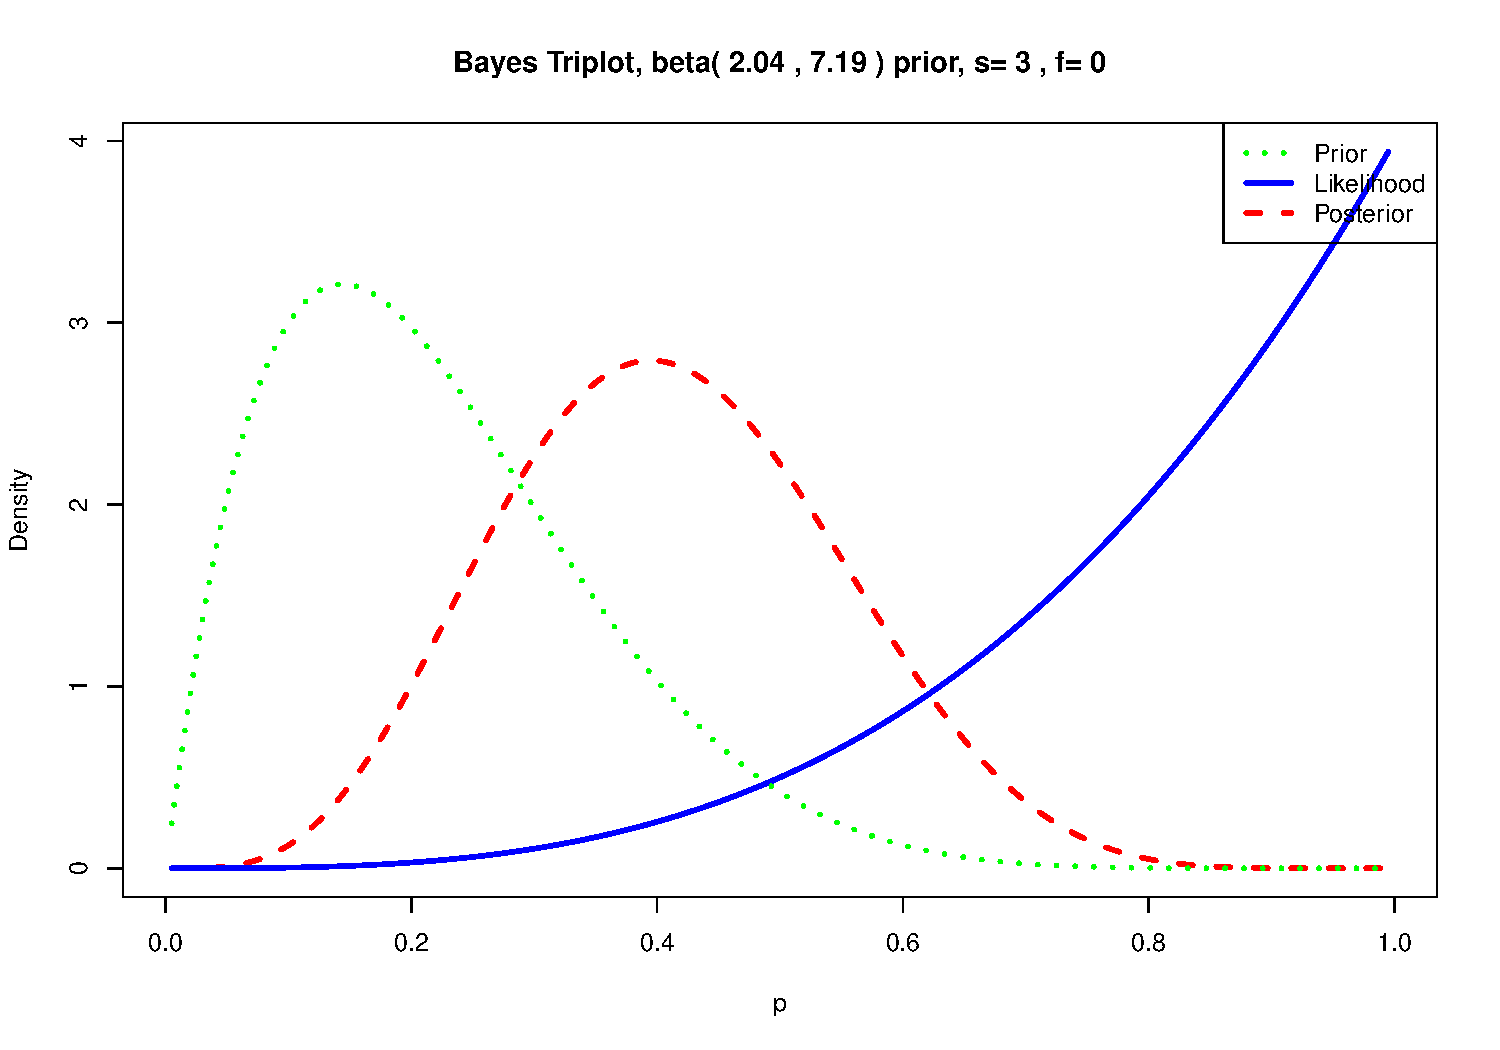
\includegraphics[scale=0.32]{05LearnBayes_files/figure-beamer/unnamed-chunk-3-1} \end{center}

\end{frame}

\begin{frame}[fragile]{Inference by sampling from the posterior}

Inference about the response rate can be carried out by simulating a
large number of draws from the posterior and summarizing the simulated
sample.

\begin{Shaded}
\begin{Highlighting}[]
\NormalTok{beta.prior =}\StringTok{ }\KeywordTok{beta.select}\NormalTok{(}\KeywordTok{list}\NormalTok{(}\DataTypeTok{p=}\FloatTok{0.5}\NormalTok{, }\DataTypeTok{x=}\FloatTok{0.2}\NormalTok{), }
\newline\KeywordTok{list}\NormalTok{(}\DataTypeTok{p=}\FloatTok{0.75}\NormalTok{, }\DataTypeTok{x=}\NormalTok{.}\DecValTok{3}\NormalTok{))}
\NormalTok{beta.post =}\StringTok{ }\NormalTok{beta.prior +}\StringTok{ }\KeywordTok{c}\NormalTok{(}\DecValTok{3}\NormalTok{,}\DecValTok{0}\NormalTok{)}
\NormalTok{post.sample =}\StringTok{ }\KeywordTok{rbeta}\NormalTok{(}\DecValTok{1000}\NormalTok{, beta.post[}\DecValTok{1}\NormalTok{], beta.post[}\DecValTok{2}\NormalTok{])}
\KeywordTok{quantile}\NormalTok{(post.sample, }\KeywordTok{c}\NormalTok{(}\FloatTok{0.05}\NormalTok{, }\FloatTok{0.95}\NormalTok{))}
\end{Highlighting}
\end{Shaded}

\begin{verbatim}
##        5%       95% 
## 0.1945582 0.6494222
\end{verbatim}

\end{frame}

\begin{frame}[fragile]{Predictive distribution}

Suppose we want to predict the number of no adverse events (successes)
in the next cohort of 3 patients.

\begin{Shaded}
\begin{Highlighting}[]
\NormalTok{beta.prior =}\StringTok{ }\KeywordTok{beta.select}\NormalTok{(}\KeywordTok{list}\NormalTok{(}\DataTypeTok{p=}\FloatTok{0.5}\NormalTok{, }\DataTypeTok{x=}\FloatTok{0.2}\NormalTok{), }
\newline\KeywordTok{list}\NormalTok{(}\DataTypeTok{p=}\FloatTok{0.75}\NormalTok{, }\DataTypeTok{x=}\NormalTok{.}\DecValTok{3}\NormalTok{))}

\NormalTok{n =}\StringTok{ }\DecValTok{3}
\NormalTok{s =}\StringTok{ }\DecValTok{0}\NormalTok{:n}
\NormalTok{pred.probs =}\StringTok{ }\KeywordTok{pbetap}\NormalTok{(beta.prior, n, s)}
\KeywordTok{discint}\NormalTok{(}\KeywordTok{cbind}\NormalTok{(s, pred.probs), }\FloatTok{0.95}\NormalTok{)}
\end{Highlighting}
\end{Shaded}

\begin{verbatim}
## $prob
## [1] 0.9763719
## 
## $set
## [1] 0 1 2
\end{verbatim}

\end{frame}

\begin{frame}{Predictive distribution}

\begin{center}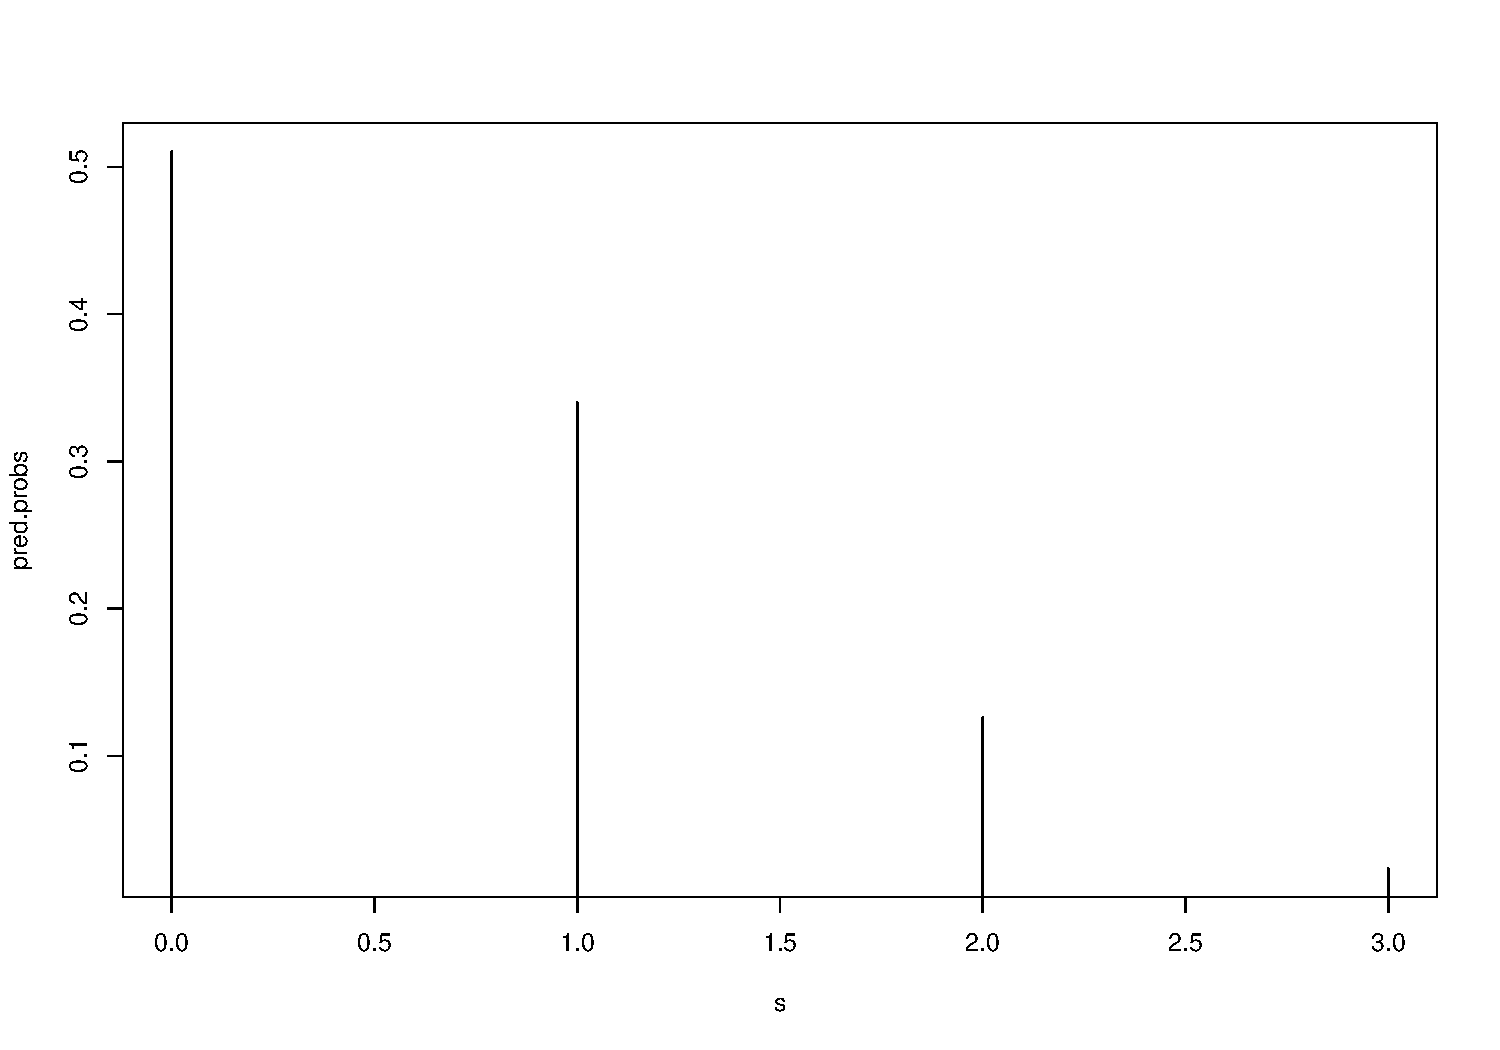
\includegraphics[scale=0.4]{05LearnBayes_files/figure-beamer/unnamed-chunk-6-1} \end{center}

\end{frame}



\end{document}